\documentclass{ctexart}
\usepackage{amsmath}
\usepackage{amssymb}
\usepackage{graphicx}
\usepackage{gbt7714}
\usepackage{wrapfig}
\usepackage{multirow}
\ctexset{
    % 修改 section。
    section={   
        name={,、},
        number={\chinese{section}}
    }
}

\title{研究弦线上的驻波现象}
\author{陆知辰-10225301456}
\date{\today}
\graphicspath{{figure/}}

\begin{document}

\begin{titlepage}
  \centering
  % 插入图片
  
\includegraphics[width=0.5\textwidth]{ecnu.png}
  
  % 空行用于调整标题位置
  \vspace*{\baselineskip}
  
  % 标题
  \Huge\textbf{物\quad 理\quad 实\quad 验 \quad (二)}
  % 空行用于调整标题和其他信息之间的间距
  \vspace*{0.3\baselineskip}
  
  % 具体实验名称
  \huge 研究弦线上的驻波现象
  
  % 空行用于调整时间和其他信息之间的间距
  \vspace*{2\baselineskip}
  
  % 时间
  \large 时间:\today
  
  % 空行用于调整时间和其他信息之间的间距
  \vspace*{\baselineskip}
  
  % 创作人
  \large 创作人:陆知辰
  
  % 空行用于调整创作人和学号之间的间距
  \vspace*{\baselineskip}
  
  % 学号
  \large 学号:10225301478
  
\end{titlepage}
\newpage
\tableofcontents
\newpage
\section{实验摘要}
  \subsection{实验概要}
  驻波是由两列传播方向相反、振幅和频率都相等,且相位差恒定的简写波叠加而成的。

  \subsection{实验目的}
  1.\quad 观察弦线上的驻波现象。

  2.\quad 研究弦线张力、振动频率、振幅三者对驻波形成的影响。
  
  3.\quad 学会如何从驻波理论出发,指定验证驻波波长和拉力、频率关系的实验方案。
  \begin{figure}[h]
    \centering
    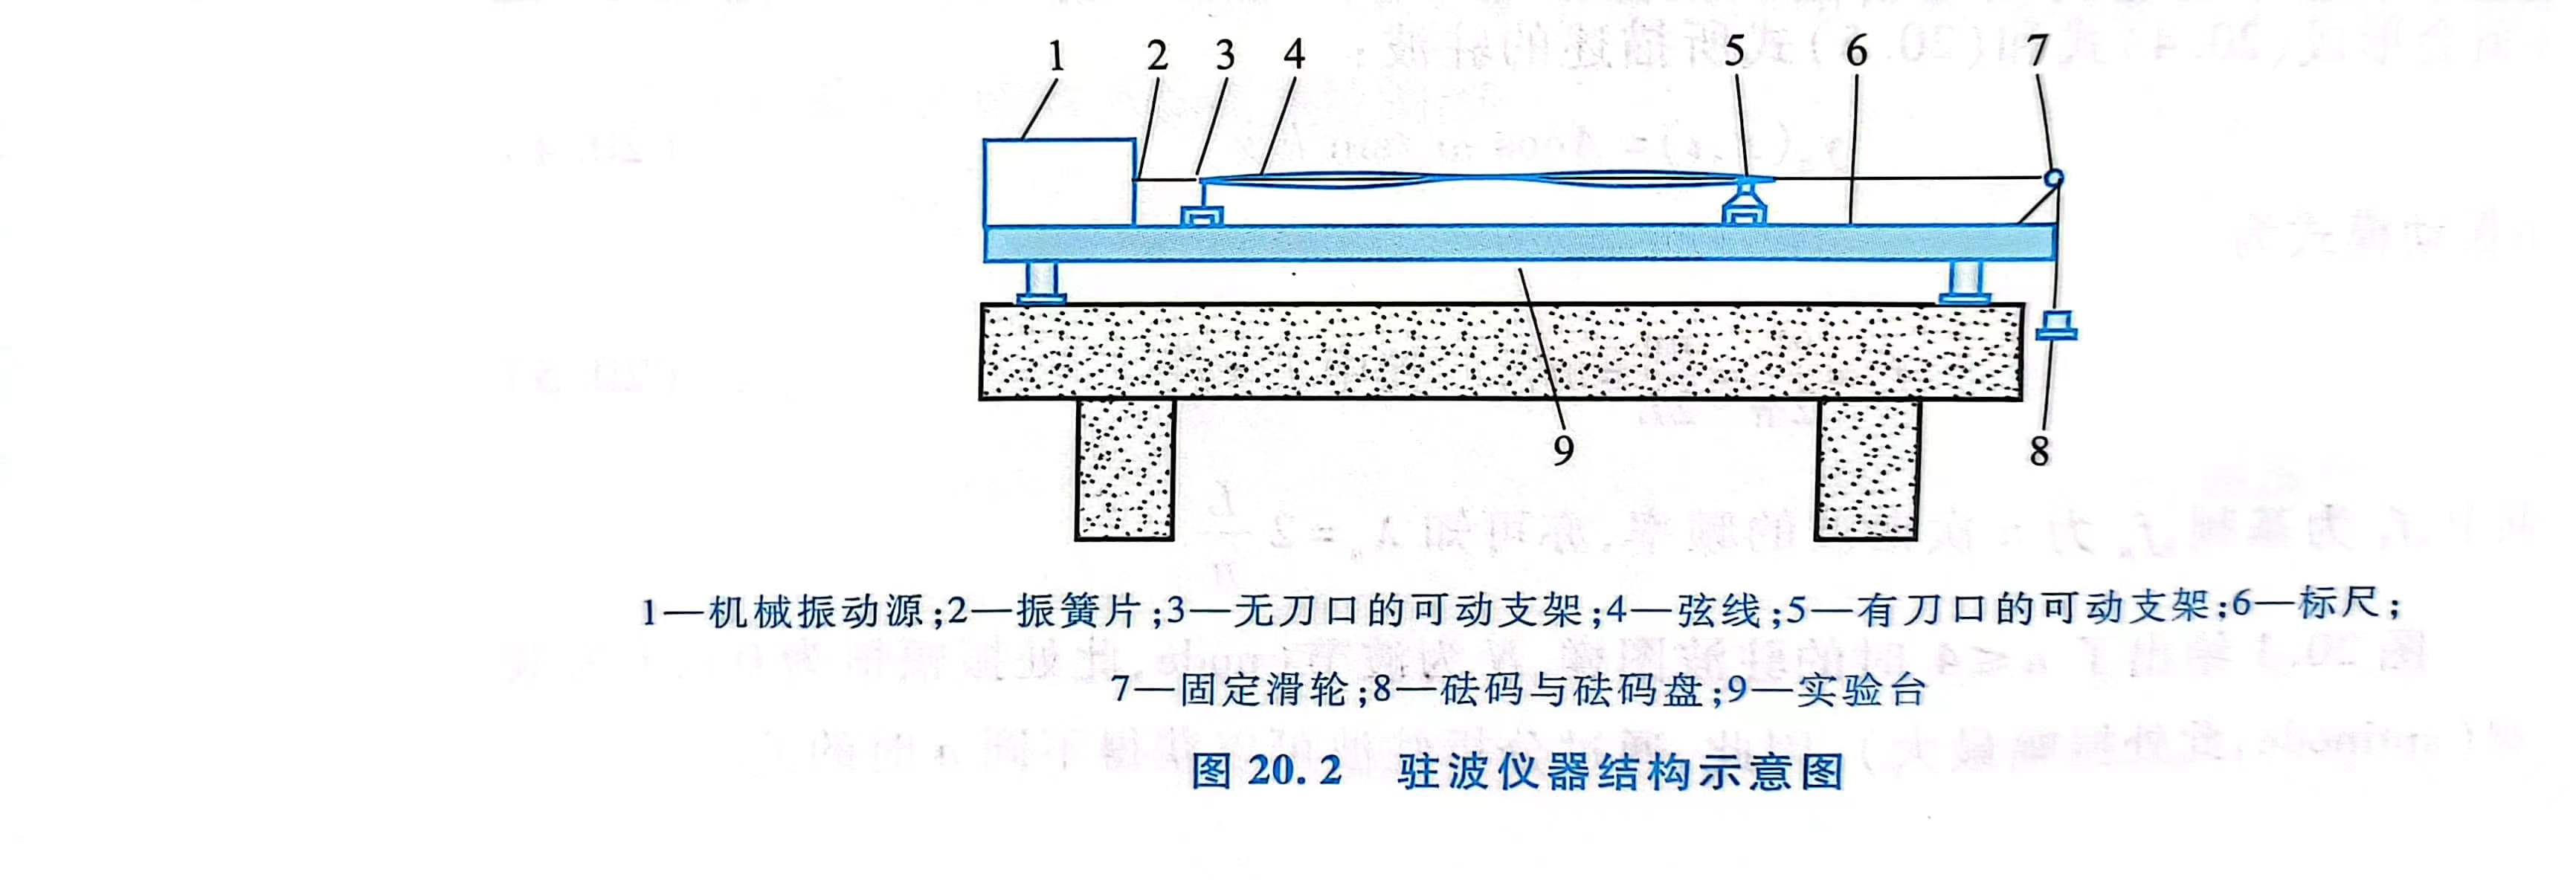
\includegraphics[height=0.4\textwidth,width=1\textwidth]{yuanli1.jpg}
    \caption{实验原理辅助用图}\label{figureyuanli1}
  \end{figure}

\section{实验原理}
实验中使用的器材如图\ref{figureyuanli1}。实验中使用该装置获得拉紧的弦线,通过振动弦线产生驻波。
金属弦线一端固定在振动源,另一端固定一个砝码。砝码能够用来使金属弦线拉紧。
同时由于刀口的存在,所以弦线无法振动,所以振动在这个位置被反射,由此形成了从右往左的波和
从左往右的反射波。在这样的条件下也能产生驻波在弦线上。

实验中将最靠近振动端的波节作为测量$L$的起始点,该点到有刀口的可动支架的距离$L$为半波长的整数倍
\begin{equation}
  L=n \frac{\lambda}{2}
\end{equation}

根据对于简谐振动的已学知识,实验中在一根拉紧的弦线上传播的机械振动横波可以被描述为
\begin{equation}\label{jixiezhendonghengbo}
  y(x,t)=A\sin ( \omega t \pm kx)
\end{equation}
在式\ref{jixiezhendonghengbo}中$y$是弦线在$x$处在$t$时刻的位移。$A$为振幅,$\omega$是振动的角频率,
$k$是角波数。对于式\ref{jixiezhendonghengbo}中出现的对象同时还应该满足波动方程
\begin{equation}\label{bodongfangcheng}
  \frac{\partial ^{2} y(x,t)}{\partial x^{2}} = \frac{1}{v^{2}} \frac{\partial ^{2} y(x,t)}{\partial t^{2}}
\end{equation}
其中$v^{2} = \frac{\omega ^{2}}{k^{2}}$

当开始振动弦线的时候,振动源会给弦线力的作用,这里假设张力为$F_{T}$,弦线的密度为$\rho _{2}$,则
可以得到弦线上沿弦线传播的横波的速度为
\begin{equation}\label{bosufangcheng}
  v=\sqrt[2]{\frac{F_{T}}{\rho _{2}}}
\end{equation}

而弦线两端固定,且长度为$L$,所以同时还需要满足振动的边界条件$y(0)=y(L)=0$,由于两端的端点是固定的,所以
传播的时候产生的波和反射波最终会相互叠加在弦线上形成驻波。驻波应该满足以下条件:
\begin{equation}\label{zhubofangcheng}
  y_{n}(x,t)=A\cos \omega _{n} t \sin k_{n} x
\end{equation}

同时还应该满足
\begin{equation}\label{zhendongmoshi}
  f_{n}=\frac{\omega _{n}}{2\pi}=\frac{nv}{2L}=nf_{1}\mbox{,其中}f_{1}=\frac{v}{2L}
\end{equation}
在式\ref{zhendongmoshi}中,$f_{1}$为基频,$f_{n}$为$n$次谐波的频率,由此可以得到
波长的表达形式为$\lambda_{n}=2\frac{L}{n}$

\begin{figure}[b]
  \centering
  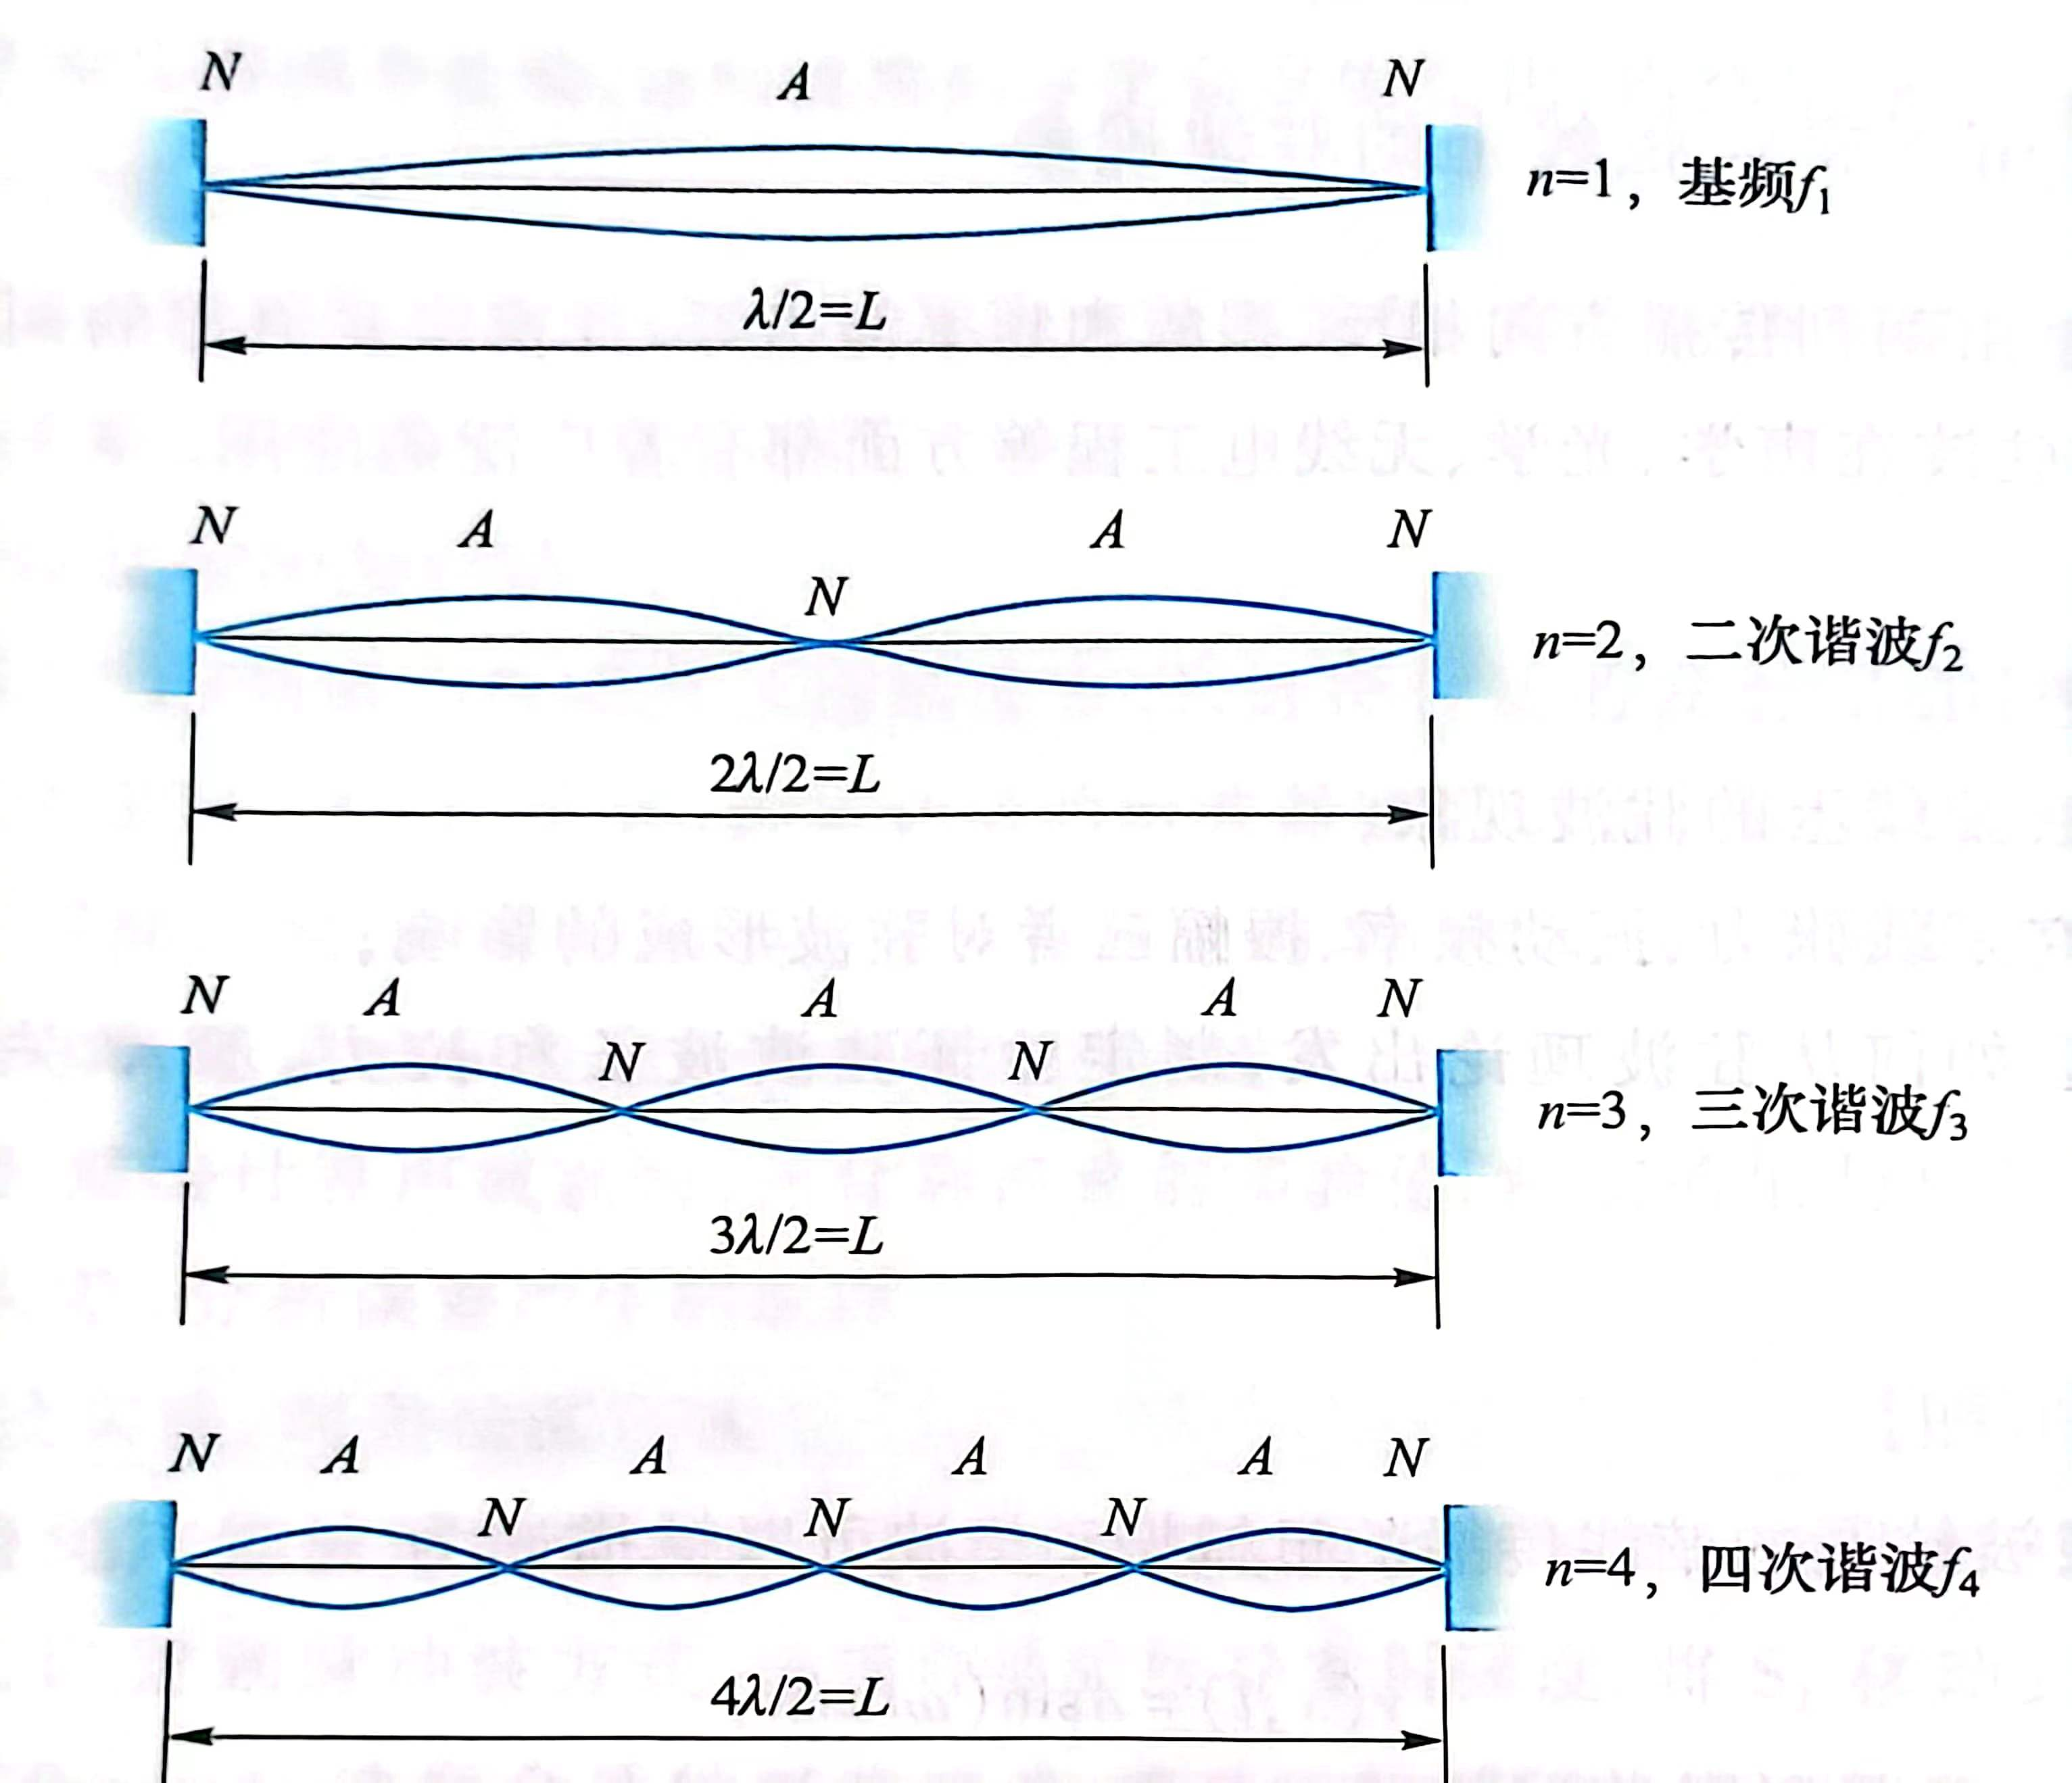
\includegraphics[height=0.3\textwidth,width=0.7\textwidth]{zhuboyanshi.jpg}
  \caption{驻波演示示意图}\label{zhuboyanshi}
\end{figure}

图\ref{zhuboyanshi}演示了在当$n\leq 4$的时候驻波的示意图像。其中$N$为波节。波节就是
振幅恒等于0的位置,$A$为波腹。波腹就是振幅最大的位置。由此图像可以直接通过观察得出$\lambda$
以及$f_{n}$表达。

根据之前得到的式\ref{bosufangcheng}能够进一步推导得出波长$\lambda$的表达形式为
\begin{equation}\label{bochangfangcheng}
  \lambda = \frac{v}{f} =\frac{1}{f}\sqrt[2]{\frac{F_{T}}{\mu}}
\end{equation}
再对式\ref{bochangfangcheng}两边取对数,就可以进一步得到
\begin{equation}\label{bochangduishufangcheng}
  \ln \lambda = \frac{1}{2} \ln F_{T}-\frac{1}{2} \ln \mu - \ln f
\end{equation}
通过式\ref{bochangduishufangcheng}可以通过实验得到数据并对数据进行
图像化处理后得到$\lambda - T$以及$\lambda -f$的图像和拟合方程。
由此验证弦线中$\lambda - T$以及$\lambda -f$的特性。

\section{实验装置器材介绍}
频率可调节的机械振动源、实验台、固定滑轮、刻度尺、不同粗细的弦线若干、
砝码盘、砝码若干、电子天平、频闪灯

\section{实验内容及实验步骤}
  \subsection{实验准备}
  实验前测量砝码的质量并记录,多次测量取平均值。并正确组装装置,保证实验中刀口能固定弦线,
  能产生反射波。
  \subsection{预实验}
  在装置组装完成后打开各项设备的开关,进行预实验。观察不同张力下的半波长出现的数量。之后调节
  机械振动源改变波动频率,观察不同波动频率下半波长出现的数量。之后调节刀口位置,左右滑动刀口的
  滑轮,观察振幅改变情况以及半波长出现的数量。

  通过预实验得到定性的结果,并定性描述弦线张力、波动频率、振幅三者对驻波形成的影响。
  \subsection{定性描述弦线张力、振动频率、振幅三者对驻波形成影响}
  结合预实验得出结果。
  \subsection{实验验证弦线张力、振动频率和波长的关系}
    \subsubsection{验证弦线张力和波长之间的关系}
    控制变量,固定振动源的频率,保证弦线上波的频率不变,改变弦线受到的拉力。
    拉力的改变通过改变砝码盘上的砝码增减来达成。每次改变张力都需要注意重新左右移动
    带有刀口的滑轮。通过移动这个滑轮来保证弦线上产生的驻波振幅较大而且稳定。

    当驻波稳定后记录振动频率、砝码质量并测量弦线上产生的驻波整数倍半波长。
    \subsubsection{验证振源频率和波长之间的关系}
    控制变量,固定弦线受到的拉力,改变振动源的频率。
    振动源频率直接对设备进行调节即可。每次改变张力都需要注意重新左右移动
    带有刀口的滑轮。通过移动这个滑轮来保证弦线上产生的驻波振幅较大而且稳定。

    当驻波稳定后记录振动频率、砝码质量并测量弦线上产生的驻波整数倍半波长。

  \subsection{实验数据处理}
  利用图像法处理波长、频率、张力有关的数据,并得出实验结论,进行总结。
\newpage

\section{实验原始数据}
\begin{figure}[h]
  \centering
  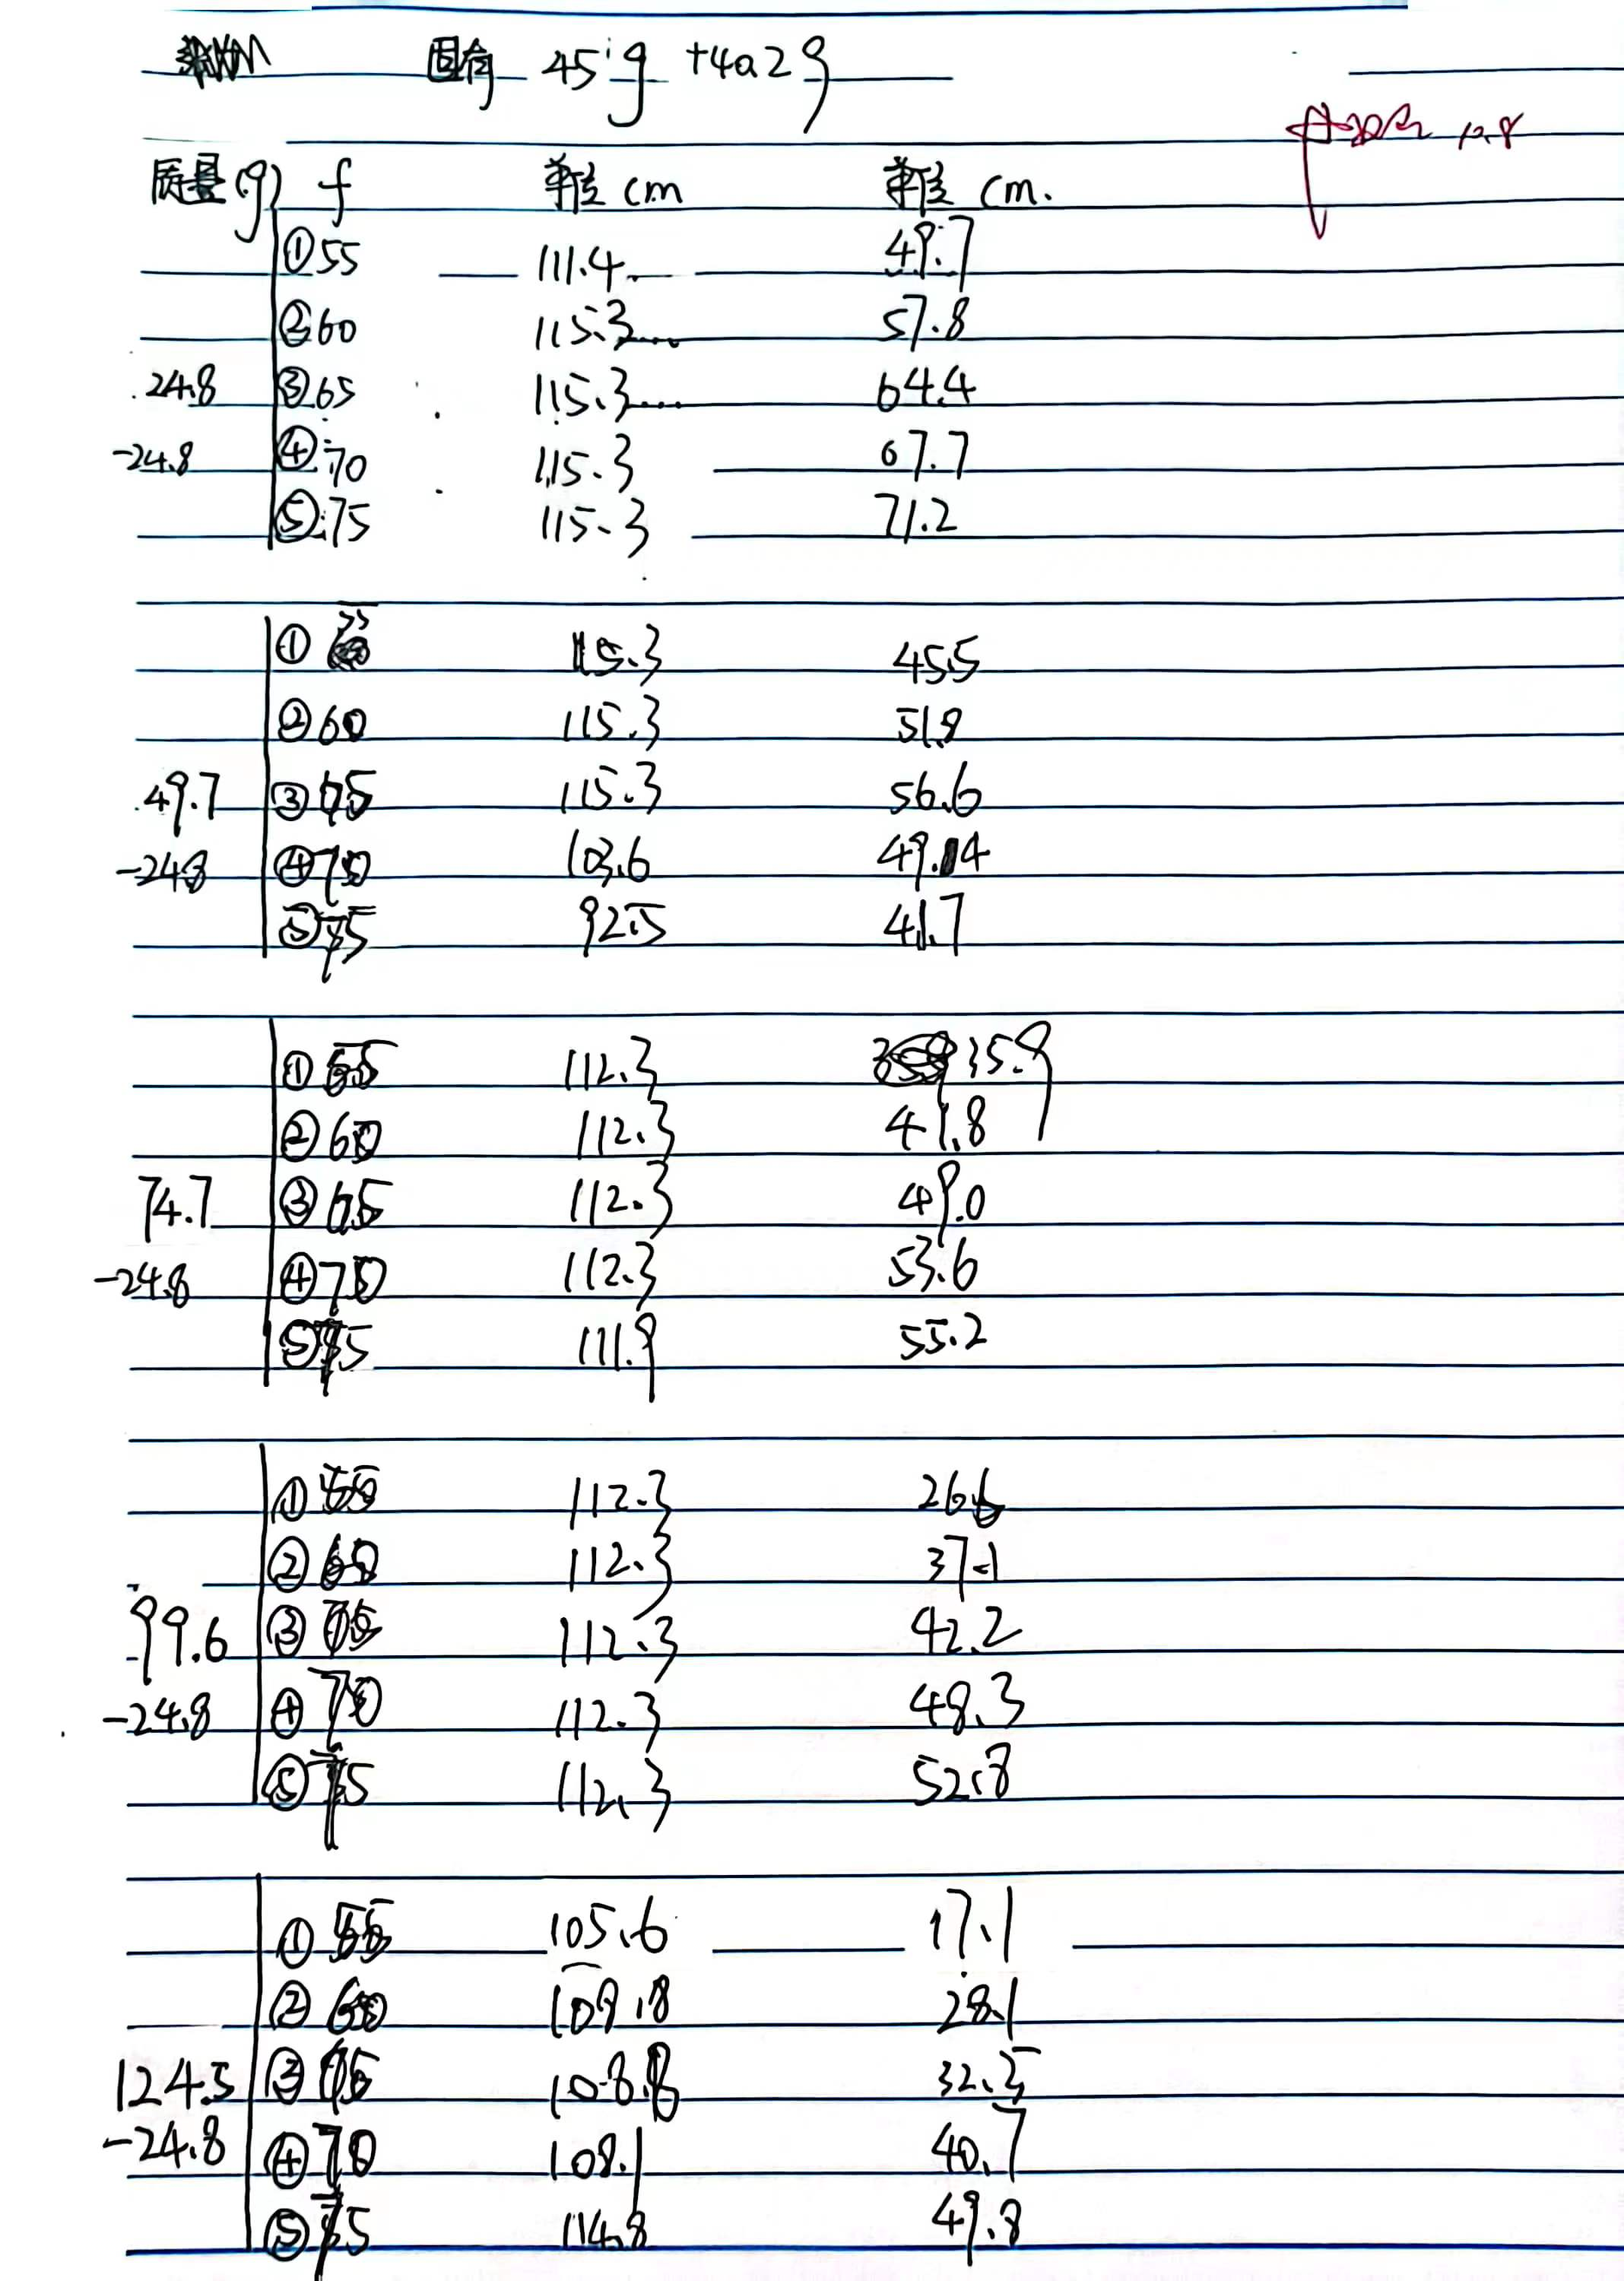
\includegraphics[height=1\textwidth,width=1\textwidth]{shiyanshujv.jpg}
  \caption{实验原始数据}\label{shiyanshujv}
\end{figure}
\newpage


\section{实验数据处理}
所用砝码情况显示如表\ref{famazhiliang},由于测量质量会引入不确定度,所以加入不确定度。
但是由于不确定量对于实验的影响较小,所以可以忽略不计。
\begin{table}[h]
  \centering   
  \caption{实验所用砝码质量及砝码盘质量}\label{famazhiliang}
  \begin{tabular}{| l || l || l |}
      \hline
      砝码 & 质量(克) & 不确定度\\
      \hline
      始终添加砝码盘 & 40.2 & $\pm$ 0.0134\\
      \hline
      始终添加的砝码 & 45.0 & $\pm$ 0.0134\\
      \hline
      选择添加砝码1 & 24.8 & $\pm$ 0.0212\\
      \hline
      选择添加砝码2 & 24.9 & $\pm$ 0.0134\\
      \hline
      选择添加砝码3 & 25.0 & $\pm$ 0.0134\\
      \hline
      选择添加砝码4 & 24.9 & $\pm$ 0.0134\\
      \hline
      选择添加砝码5 & 24.9 & $\pm$ 0.0212\\
      \hline                       
  \end{tabular}
\end{table}

实验原始数据数字化后结果如图\ref{shiyanshujvexl}
\begin{figure}[h]
  \centering
  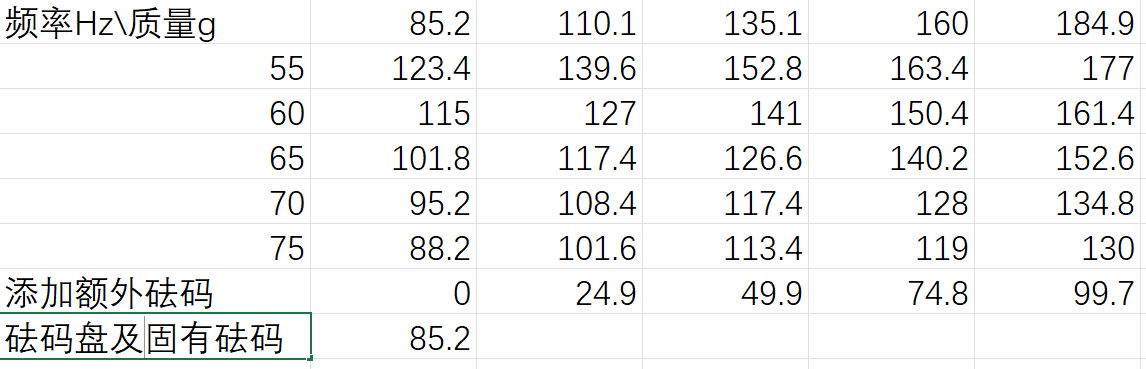
\includegraphics[width=1\textwidth]{shiyanshujvexl.png}
  \caption{实验原始数据数字化结果}\label{shiyanshujvexl}
\end{figure}

  \subsection{验证弦线张力和波长之间的关系}
  \begin{figure}[b]
    \centering
    \begin{minipage}[b]{0.48\textwidth}
      \centering
      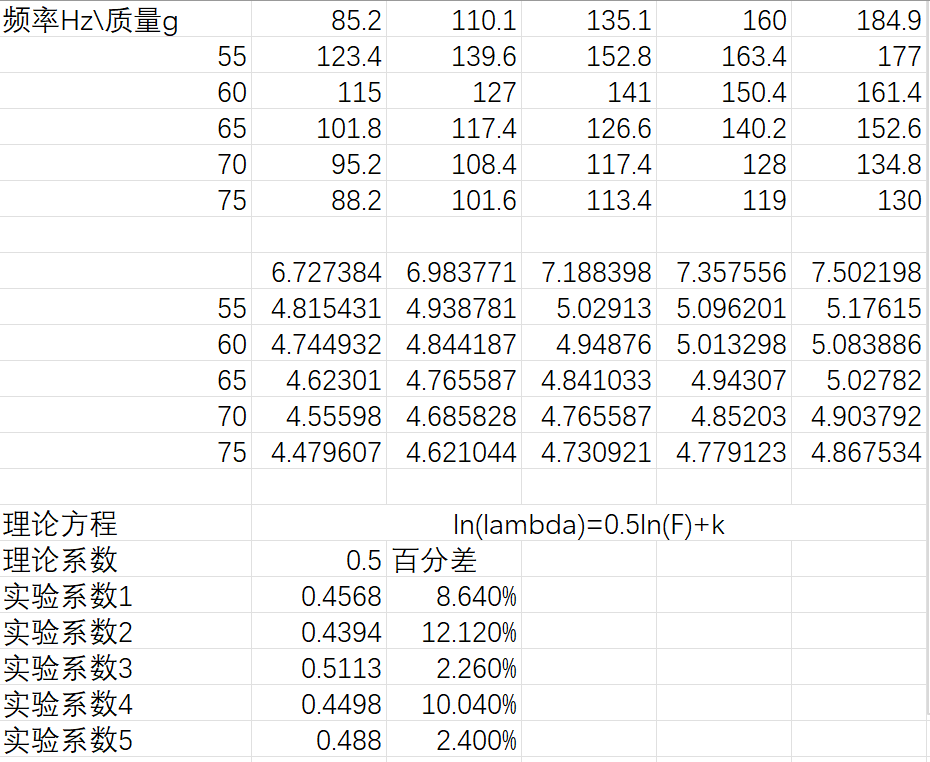
\includegraphics[width=0.46\textwidth]{yanzhengzhanglishujv.png}
      \caption{验证弦线张力和波长之间的关系数据}\label{yanzhengzhanglishujv}
    \end{minipage}
    \begin{minipage}[b]{0.48\textwidth}
      \centering
      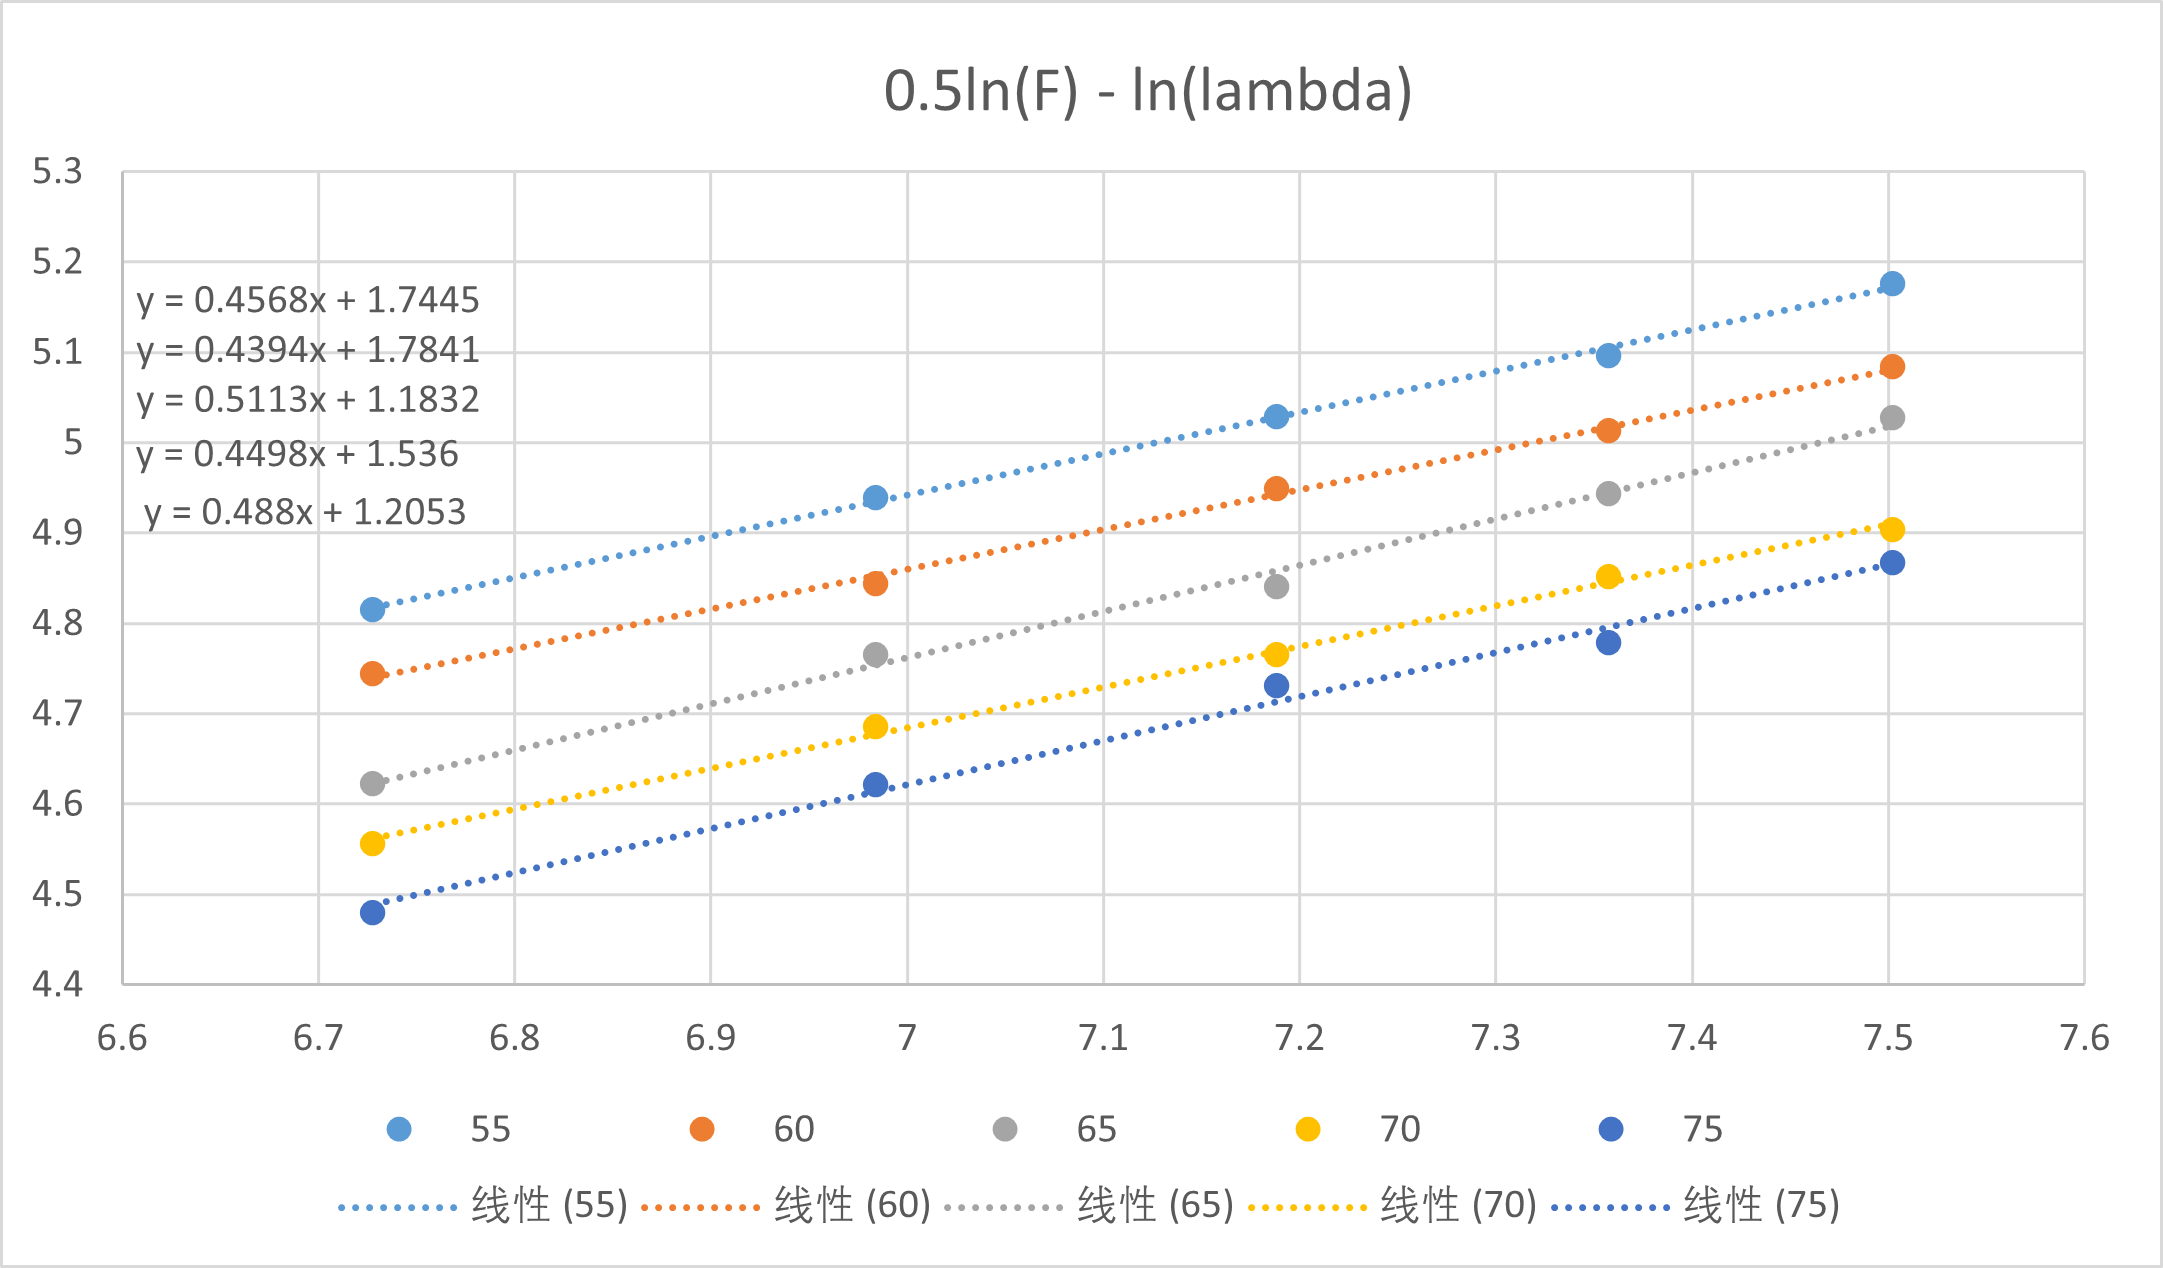
\includegraphics[width=0.46\textwidth]{yanzhengzhanglizuotu.png}
      \caption{验证弦线张力和波长之间的关系作图}\label{yanzhengzhanglizuotu}
    \end{minipage}
  \end{figure}

  实验数据处理如图\ref{yanzhengzhanglishujv},实验作图如图\ref{yanzhengzhanglizuotu}。

  根据实验原理中获得的公式,即式\ref{bochangduishufangcheng}可得
  $$\ln \lambda = \frac{1}{2} \ln F_{T}-\frac{1}{2} \ln \mu - \ln f$$
  所以对于波长$\lambda$和张力$F_{T}$两者关系进行数据处理,并运用作图法,最终得到的拟合方程
  应该满足:\\
  1. 形式上满足一次函数形式,即$y=kx+b$\\
  2. 具体参数上自变量前的系数应等于0.5

  最终得到的方程以及系数结果和理论值的百分差如表\ref{yanzhengzhanglibaifencha}
  \begin{table}[h]
    \centering   
    \caption{验证弦线张力和波长之间的关系结果}\label{yanzhengzhanglibaifencha}
    \begin{tabular}{| l || l || l |}
        \hline
        理论值 & 实验值 & 百分差\\
        \hline
        \multirow{5}{*}{0.5} & 0.4568 & 8.64\% \\
        \cline{2-3}
        & 0.4394 & 12.12\% \\
        \cline{2-3}
        & 0.5113 & 2.26\% \\
        \cline{2-3}
        & 0.4498 & 10.04\% \\
        \cline{2-3}
        & 0.4880 & 2.40\% \\
        \hline                   
    \end{tabular}
  \end{table}

  由最终结果可以看出实验中数据的误差差距较大,最高百分差达到12.12\%,而最小百分差只有2.26\%。
  实验中的误差可能来源于:

  1、记录波长的时候波节位置寻找的误差。

  2、虽然形成了稳定的驻波,但是由于器材灵敏度并不高导致形成并不是完美的共振但是肉眼无法识别。

  3、实验数据涵盖范围可以进一步扩大,涵盖更大范围的情况减少误差。

  4、虽然实验中使用了刀口作为端口,但是弦线依旧会产生左右或者上下的晃动,导致张力维持不稳定出现误差。

  \subsection{验证振源频率和波长之间的关系}
  \begin{figure}[b]
    \centering
    \begin{minipage}[b]{0.48\textwidth}
      \centering
      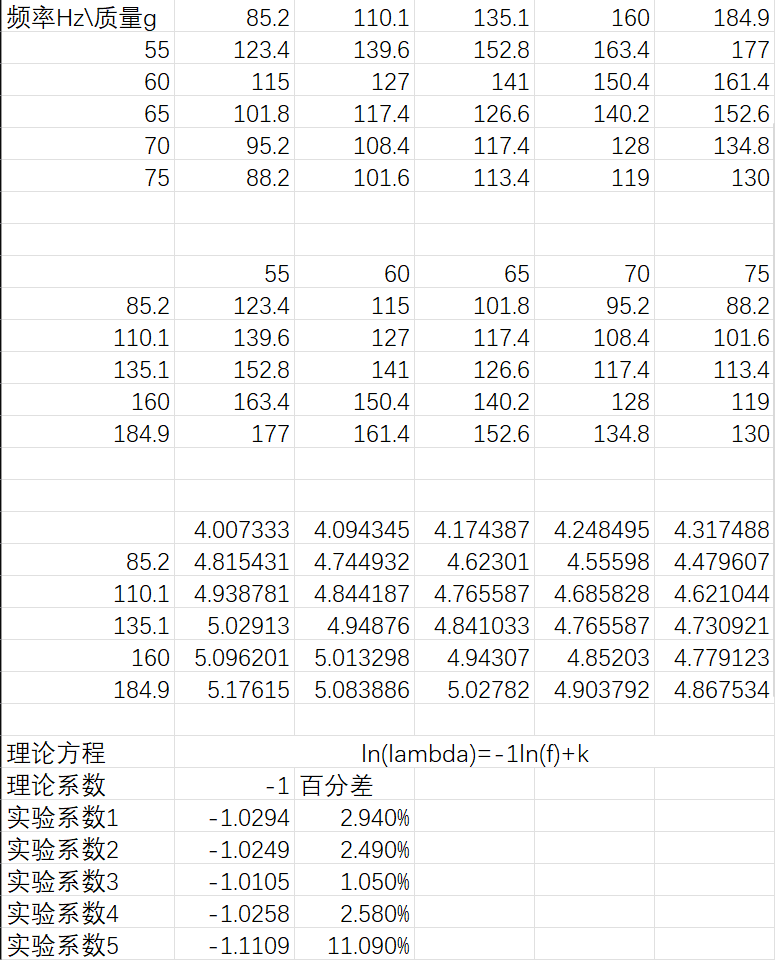
\includegraphics[width=0.46\textwidth]{yanzhengpinlvshujv.png}
      \caption{验证振源频率和波长之间的关系数据}\label{yanzhengpinlvshujv}
    \end{minipage}
    \begin{minipage}[b]{0.48\textwidth}
      \centering
      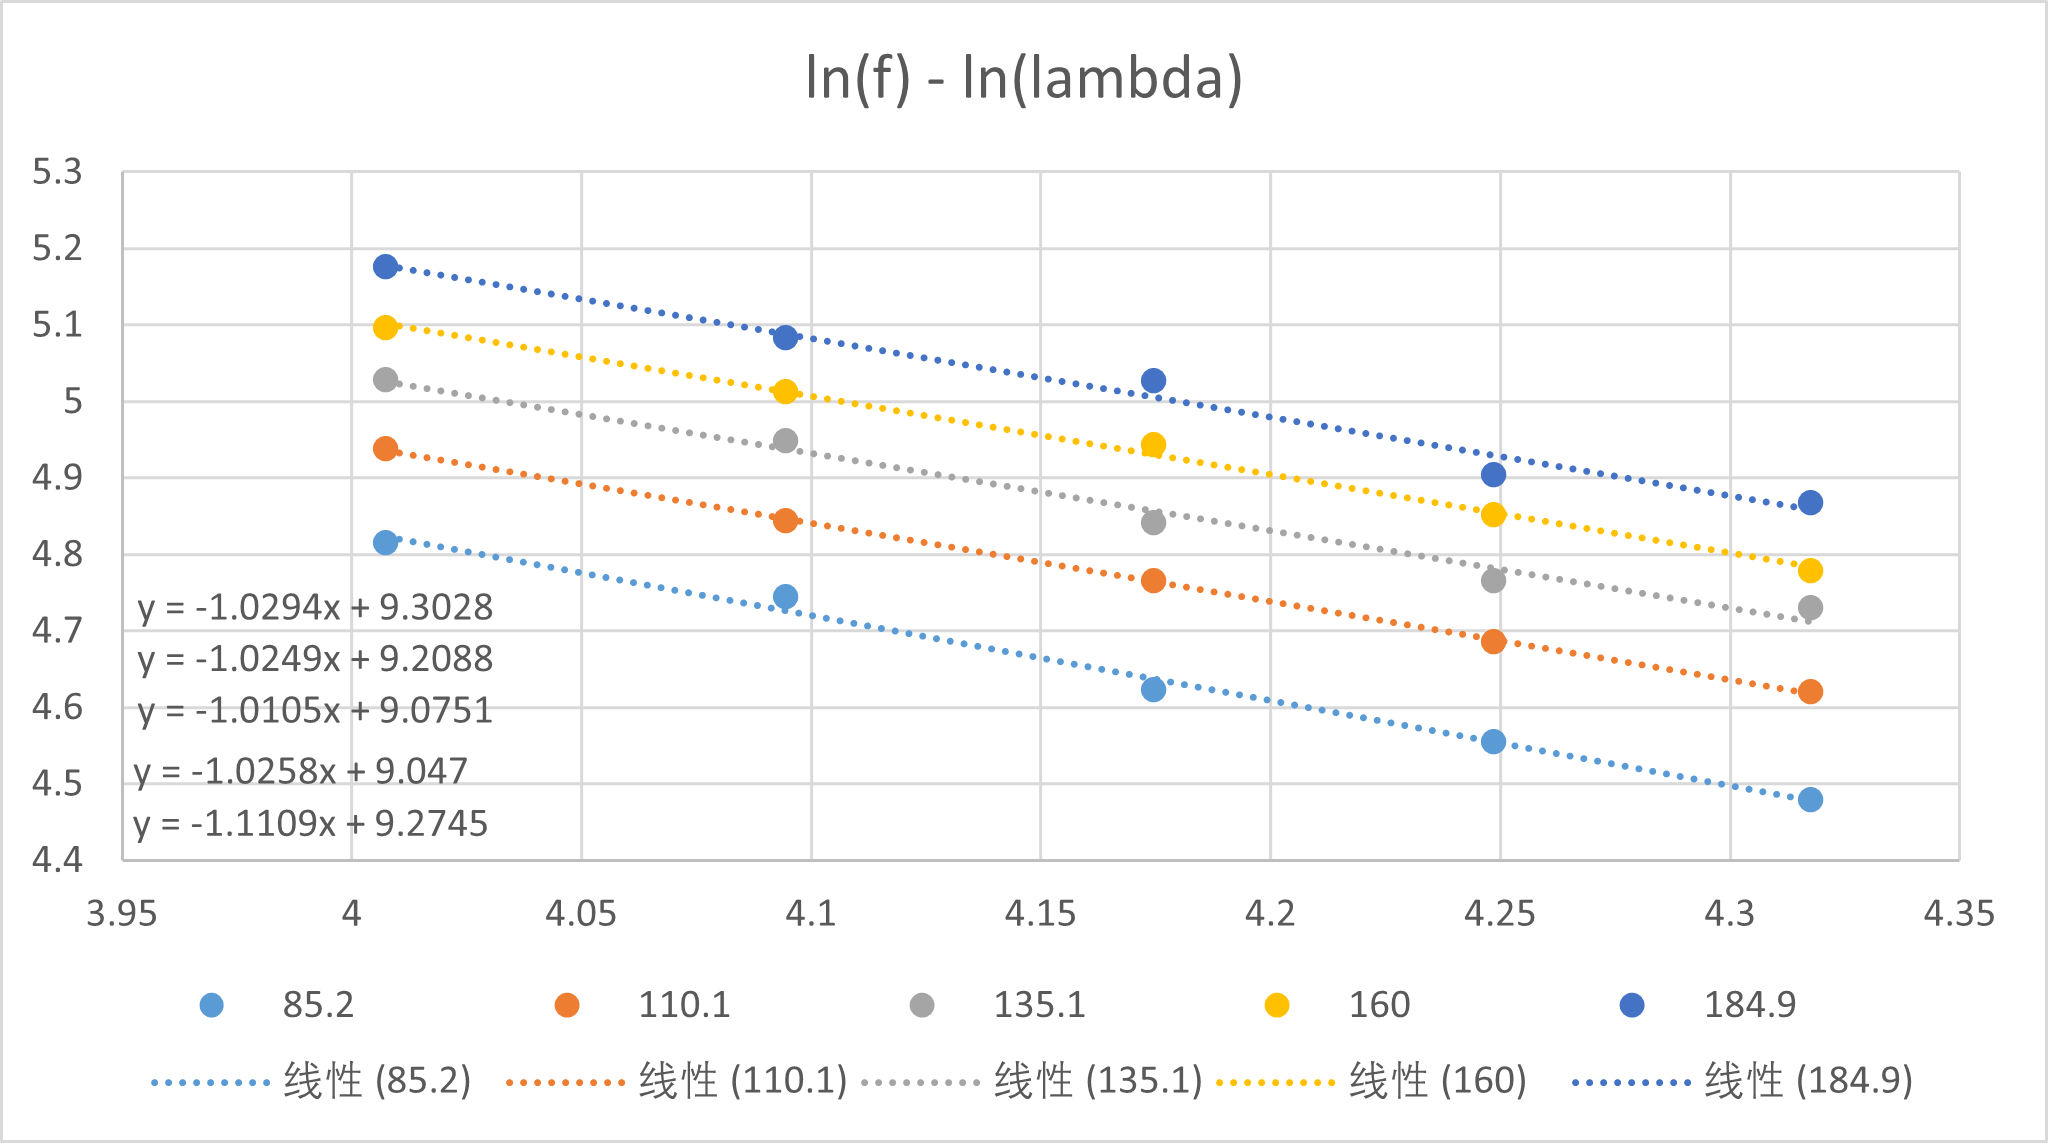
\includegraphics[width=0.46\textwidth]{yanzhengpinlvzuotu.png}
      \caption{验证振源频率和波长之间的关系作图}\label{yanzhengpinlvzuotu}
    \end{minipage}
  \end{figure}

  实验数据处理如图\ref{yanzhengpinlvshujv},实验作图如图\ref{yanzhengpinlvzuotu}。

  根据实验原理中获得的公式,即式\ref{bochangduishufangcheng}可得
  $$\ln \lambda = \frac{1}{2} \ln F_{T}-\frac{1}{2} \ln \mu - \ln f$$
  所以对于波长$\lambda$和张力$F_{T}$两者关系进行数据处理,并运用作图法,最终得到的拟合方程
  应该满足:\\
  1. 形式上满足一次函数形式,即$y=kx+b$\\
  2. 具体参数上自变量前的系数应等于-1


  最终得到的方程以及系数结果和理论值的百分差如表\ref{yanzhengpinlvbaifencha}
  \begin{table}[h]
    \centering   
    \caption{验证振源频率和波长之间的关系结果}\label{yanzhengpinlvbaifencha}
    \begin{tabular}{| l || l || l |}
        \hline
        理论值 & 实验值 & 百分差\\
        \hline
        \multirow{5}{*}{-1} & -1.0294 & 2.94\% \\
        \cline{2-3}
        & -1.0249 & 2.49\% \\
        \cline{2-3}
        & -1.0105 & 1.05\% \\
        \cline{2-3}
        & -1.0258 & 2.58\% \\
        \cline{2-3}
        & -1.1109 & 11.09\% \\
        \hline                   
    \end{tabular}
  \end{table}

  由最终结果可以看出实验中数据的误差差距较大,最高百分差达到11.09\%,而最小百分差只有1.05\%。
  实验中的误差可能来源于:

  1、记录波长的时候波节位置寻找的误差。

  2、虽然形成了稳定的驻波,但是由于器材灵敏度并不高导致形成并不是完美的共振但是肉眼无法识别。

  3、实验数据涵盖范围可以进一步扩大,涵盖更大范围的情况减少误差。

  4、虽然实验中使用了刀口作为端口,但是弦线依旧会产生左右或者上下的晃动,导致张力维持不稳定出现误差。
\newpage

\section{思考题}
  \subsection{频闪仪的作用}
  实验中并没有使用到频闪仪。但是根据名称以及对于实验器材的了解,频闪仪的作用应该是帮助观察驻波形成的
  实验道具。由于如果直接通过肉眼进行观察的话,受限于人类眼睛能观察的最大采样率,导致观察驻波会非常苦难。
  而且如果实验室的光线环境不够适宜更难进行观察。所以使用频闪仪。频闪仪一方面能照亮实验器材,另一方面能够
  让驻波在视觉上处于不动稳定的状态,最大程度减小弦线振动残影产生的影响。

  \subsection{确定弦线上的波节点的位置方法}
  实验中由于没有使用频闪灯,对于波节的确定也只能使用肉眼观察。在一段观察中表现为静止的部分取中点作为波节。
  理论上,实验中波节应该为振动为0的点,也就是没有发生振动的点。但是实验中由于振幅本身就不大,所以显得波节非常
  难以确定。

  至于为什么使用中点,因为视觉上不震动的一段,由于波的周期性,所以驻波也具有对称性,所以中点更加接近真实的
  波节的位置。
  \subsection{调节振动源的振幅大小对弦线振动产生的影响}
  调节振动源振幅对于弦线振动的频率没有影响,因此也不会影响波长。振幅的大小会直接影响实验中观测到现象的
  明显程度。更大的振幅更容易观测到波节位置,也更容易确定驻波是否形成。但是振幅过大同样也会导致实验问题出现。
  过大的振幅可能导致实验中弦线的断裂,尤其在添加多个砝码,弦线的张力变大的时候。
\newpage

\section{实验中个人的思考与感想}
  \subsection{对于实验个人观点和感想}
  实验需要研究的是驻波的波长和振动频率以及弦线张力的关系。使用的方法也是控制变量法。但是实验操作中仍然会出现一定问题。

  首先实验中使用的振动源的振幅在高频率下并不是非常大,这也导致实验中可能形成的驻波的振幅不够明显,对于确定驻波的波节
  会产生影响。

  其次,实验中没有考虑到物体的固有频率。$\mbox{固有频率}^2 = \frac{1}{4\pi^2} \frac{\mbox{刚度}}{\mbox{质量}}$
  在实验中50-60Hz的频率下振动非常剧烈,可能会和这个有关。

  最后,还有一个很有趣的现象,就是在调节频率的时候如果调节的速度非常快那几乎就无法显示出驻波。分析因为驻波形成需要
  时间也需要能量,快速调节频率的时候没有足够能量能够形成驻波,只有当调节频率中稍微停顿才会出现驻波。

  \subsection{实验中的总结}
  实验的设计非常简单,基本就是按照需要控制变量进行的,而且变量也不多,只有两个。但是在实际操作中仍然会出现很多问题。
  实际实验中会出现很多误差或者操作问题导致实验最终结果和理想结果相差较大。
\end{document}